% Template PNSAC newsletter - Article
% Language: Latex
%

% Head

\title{Diversion to Alert}
%\subtitle{Part 4}
\author{Malcolm G. Morrison, RCAF F/L Ret.}

\maketitle

%\end{multicols}

%\begin{figure*}[htbp]
%	\vspace{2em}
%	\centering
%	%name of the graphic, without the path AND in EPS format:
%	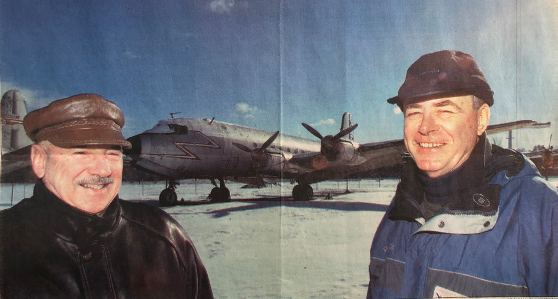
\includegraphics[scale=0.8]{holmgren-timmin-scaled.png}
%	%caption of the figure 
%	\caption*{\small \em TIm Timmins, left, and Robert Holmgren are forming a
%group of skilled volunteers to restore a 55-year-old North Star, the first
%Canadian-made plane capable of transcontinental flight.}
%	%label of the figure, which has to correspond to \ref{}:
%	\label{fig:timmins-holmgren}
%\end{figure*}


%\begin{multicols}{2}

\textit{This article was published in Air Force Magazine in April 2019. It was
brought to our attention by Gary Whitten. The article is republished
with the express permission of Malcolm Morrison, RCAF F/L Ret. and the
publishers of Air Force Magazine.}\\

Immediately after New Year 1960, while based at RCAF Stn Trenton, and
flying North Stars for 426(T)Sqn., I was assigned to be the First
Officer on a flight to pick up an entertainment troupe of 30 Passengers
from Montreal. This was planned as an 8 day trip providing
entertainment to personnel working along the Quebec, Ontario and
Manitoba sectors of the Mid Canada Detection Line.

At the height of the Cold War, The Mid Canada Line was to be the main
detection line between Canada and the USSR. It was located
approximately along the 55N latitude parallel, and stretched from
Hopedale, Labrador to Dawson Creek, B.C. The system was put into
service in 1957, and decommissioned in 1964. The more northerly DEW
radar line began full operation in 1957.

Our 426Sqn crew consisted of Captain – F/O H.(Hank) Zbesheski, First
Officer – F/O M.G.(Mac or Mo) Morrison, Navigator – F/O Roger Fridel,
Radio Officer – F/O Peter Dragovich, Flt Engineer – Sgt Miller, Flt
Engineer – Sgt Sopaz, Trans Tech – LAC Hall.

It should be noted that, on northern flights such as this, it was
normal to have two Flight Engineers on the crew, due to the difficulty
of fueling and servicing the North Star in remote and unsupported
airfields. Had there been plans to travel north of Churchill, we would
normally carry an extra navigator as well. Another part of the Squadron
normal operating procedure was that; providing the First Officer was
Type qualified and current, the Captain and First Officer would switch
seats on alternate legs. The North Star did not have nose wheel
steering available in the co-pilot's position.

Typically, on the day prior to departure from home base the whole crew
would meet and review the trip Itinerary, and fully discuss any
foreseen issues that might be expected. We were all aware of the
anticipated cold weather, the short snow packed runways at most of the
planned stops, and the lack of any useable hangar facilities that could
accommodate a North Star, with the exception of RCAF Churchill.

Having introduced the issue of cold weather, I must now digress for a
moment to explain one of the severe consequences of cold weather on
aero engines in 1960.   At ambient temperatures below minus 18 deg. C,
90w oil is below its "pour point"; in other words it would not flow
through either a filter or a radiator such as the type required to cool
the oil on the North Star. Each engine had a 25 gal oil tank located in
the wing immediately behind the engine firewall. To ensure that the oil
system worked after a prolonged (30 to 40 minute) engine shut down in
temperatures below minus 18 deg. C, the requirement was to dilute the
oil with raw gasoline directly from the main fuel system. As an example
at a temperature of minus 34 C the dilution time was approximately 3
minutes when the oil temperature had cooled to 40 deg. C. After
start-up the next morning the gasoline had to be boiled out of the oil
for approximately 35 minutes once the oil had reached a
40degC.temperature.

These procedures were called "oil dilution" and oil "boil-off". The
dilution and boil off times which I have cited are approximations only,
since I have not had access to the Standard Operating Procedures for
the North Star for quite some time.

The reason for dwelling on the oil dilution procedures is that, in
January of 1962, North Star \#17520 operated by 412 Sqn. was lost at Hall
Beach NWT, during a VIP tour of Dew Line sights. Within minutes of
takeoff from Hall Beach in minus 40C conditions, the crew experienced 3
engine failures in rapid succession. Under very difficult conditions,
they were able to force land the aircraft on the infield of the
airport. Fortunately, all passengers and crew were able to exit the
aircraft without injury. On a subsequent trip in April of 1964 doing a
similar Dew Line site tour in \#17502, I witnessed the remains of 17520
still sitting in the infield, a stark reminder of oil dilution
requirements.

To continue with my story, with the exception of St. Hubert and
Churchill, there were no stairs available to board or deplane our
passengers on, and thus the passengers were required to climb down a
rather slim aluminum ladder each time. This process could amount to
more than a 30-minute exercise each time, and in those temperatures
this raised the oil dilution issue. We fully briefed on oil dilution
procedures prior to shut-down, and burn-off times that would be
required after engine startup and warmup the following morning. It was
agreed that, in spite of the extended periods, the passengers would be
required to board and remain seated, during the boil-off period prior
to take-off, and that we would perform both the dilution and boil-off
while the passengers were on board the aircraft.

Our planned itinerary was as follows:

\begin{itemize}
  \item 8 Jan---Trenton to St. Hubert to Sept Iles PQ---overnight at RCAF Stn
Moisie 
  \item 9 Jan---Sept Iles to Knob Lake---overnight at RCAF Stn Knob Lake
  \item 10 Jan---Knob Lake to Great Whale PQ---overnight at RCAF Stn Great
Whale River 
  \item 11 Jan---Great Whale to Winisk ON---overnight at RCAF Stn
Winisk 
  \item 12 Jan---Winisk to Churchill MB---three overnights at RCAF Stn
Churchill 
  \item 15 Jan---Churchill to St Hubert to Trenton
\end{itemize}

RCAF Stn Moisie was not part of the Mid Canada Line but was part of the
original Pinetree line. The airport at Sept Iles was not part of RCAF
Moisie, but was managed by the Federal Department of Transport. The
airports along the Mid Canada Line, although used by some civilian
contractors, were all operated by the RCAF.

The schedule, as planned, was to arrive at each of the entertainment
destinations in the late afternoon so that the Troupe could have supper
and then prepare for a show at approximately 8pm each evening. The
exception would be the days at Churchill, during which time the Troupe
would travel for 4 to 5 hours via train from Churchill to RCAF Stn
Bird, about 180 mi. to the south, entertain the base personnel, and
return to Churchill the following day.

As they say "all the best laid plans of mice and men", something is
bound to cause a SNAFU. The following is an account of what happened,
in the best chronology that my memory and my log book records can
account for.\\

\noindent\textbf{Day 1, 8 Jan 1960, North Star \#17502:}\\

The flight from Trenton to St. Hubert was uneventful, and our
passengers had already arrived, so that there was a minimum of delay in
boarding. The fuel load was topped up to the maximum that we could
carry, bearing in mind that fuel at Sept Iles would have to be
purchased on a DPO (detached  purchase order) at a significantly higher
cost than normally paid by the RCAF. We also tried to minimize the fuel
requirements at the Mid Canada sites due to the need to use fuel cache
supplies from barrels at those destinations.

The 3:05 hour flight to Sept Iles was also uneventful, with the arrival
being in darkness and in a light snowfall. Our passengers deplaned, via
the ladder, to an awaiting bus after remaining seated on board the
aircraft while the crew carried out the mandatory oil dilution
procedure prior to securing the aircraft for the night.\\

\noindent\textbf{Day 2, 9 Jan 1960, North Star \#17502:}\\

The planned chock to chock time for the leg Sept Iles to Knob Lake was
1:15 Hrs., but was logged as 2:00 Hrs., because of the engines on to
engines off time required to accommodate the boil off and dilution
procedures. The flight was uneventful; however, the landing in calm
wind conditions on a 4,500 ft. runway and with the extra fuel load was,
to say the least, challenging. The packed snow condition did not offer
good braking action.\\

\noindent\textbf{Day 3, 10 Jan 1960, North Star \#17502:}\\

The overnight temperature dropped to minus 40C as was forecast, and by
noon had not gone up appreciably. The passengers were loaded onto an
ice-cold aircraft and told that it would be at least 40 minutes before
we could commence our take off and thus turn on the main cabin heaters.
They were told that they could come into the crew area 3 or 4 at a time
and share what heat came off the cockpit heater (which had a blower
attached to it), and do that until such time as we had finished the
boil-off prior to take-off.

The engine start-up sequence on the North Star was normally 3-4-2-1.
Startup in cold weather was always tricky, in that the amount of
priming time recommended was not clearly defined in the SOP's other
than to say that, if you over-primed, you may damage the engine on
start or, if you under-primed, the engine may not start, and the
starter may be damaged by over-cranking.

We were lucky with the \#3 \& \#4 starts, but when we got to \#2, our luck
ran out and we had a severe backfire on startup, thus making the engine
totally unserviceable.

After unloading our passengers and advising them that, if they wished
to put on another show for the base personnel that afternoon or
evening, there would be no problem as far as our crew was concerned,
and that we would advise them later in the day as to what the plan
would be going ahead. We immediately advised ATCHQ as to our problems,
and were advised a few hours later that another North Star with a
replacement engine was being dispatched that afternoon, and would be
expected in the early evening. The plan was that the engine change
would take place overnight, and that our crew would carry on the next
day using the replacement aircraft and complete the Mid Canada Line
tour.

Sure enough, about 1800Hrs local time North Star \#17512 landed at Knob
Lake with a few extra technicians to assist with the engine change. The
next 6 to 7 hours were probably one of the most challenging that our
flight engineers had ever faced. With a minus 43C temperature, no
hangar facility, and virtually no support equipment, other than a 6,000
lb. forklift, these professionals, with some assistance from the rest
of our two crews, carried out the miracle of a complete engine change,
and the loading of the damaged engine onto \#17502. They also started
the replacement engine and carried out an oil dilution on the new
engine, so as to be safe for an overnight stay.

The reason for our crew and passengers not carrying on with \#17502 was
the requirement to "air test" the aircraft after an engine replacement.
This air test could not be done with passengers on board. The crew
returning 17502 to Trenton with the unserviceable engine on board
carried out the required "air test" enroute.\\

\noindent\textbf{Day 4, 11 Jan 1960, North Star \#17512}\\

The 2:50 Hr. flight from Knob Lake to Great Whale River was uneventful.
The passengers survived the 50 min. warm up and boil off period prior
to takeoff with admirable patience. On arrival at Great Whale, the
temperature of minus 29C mandated another oil dilution prior to
shut-down and deplaning.\\

\noindent\textbf{Day 5, 12 Jan 1960, North Star \#17512}\\

A short hop from Great Whale to Winisk of 1 hour flight time was logged
as 1:50 Hrs. "engines on" to "shutdown". By this time our passengers
had fully accepted the necessity of the extra wait on the aircraft. The
flight was uneventful.\\

\noindent\textbf{Day 6, 13 Jan 1960, North Star \#17512}\\

When the crew appeared at the mess hall for breakfast, we were handed a
very brief "Confidential " message from ATCHQ advising us to advance
our planned departure as much as possible, proceed to Churchill,
deplane our passengers, refuel and proceed immediately to Winnipeg
where we would be given further instructions.

Following a 2:20 hour flight to Churchill we advised our passengers
that we had to proceed to Winnipeg immediately, but would be back to
pick them up and return them home in three days. The 3:10 hour flight
to Winnipeg was uneventful, with arrival being after dark. The aircraft
was immediately towed into a hanger with the instructions that we could
refuel in the morning when we had been fully briefed on our future
mission.

As the crew deplaned we were met by an army major and taken to a
briefing room, where we were told the "Confidential" details of our
diversion. The following is a short synopsis of that briefing. We were
to get a good night's sleep, and first thing in the morning we would be
given a full briefing on the perils and extreme hazards that a 15 drum
load of "specially denatured alcohol 3C, 200 proof" would create on an
"emergency flight" to CFB Alert the next morning.

The planned route was Winnipeg to Churchill, Resolute Bay and Alert,
unload, and on to USAF base Thule in Greenland for a crew rest. It was
agreed that Nav. F/O Fridel was well enough versed in grid navigation
to eliminate the requirement for a second navigation officer.  We were
advised that sufficient food would be provided to see us through to
Thule, and that both Churchill and Resolute would be alerted as to the
urgency of our mission, and would give us all the required assistance
for quick turn-around at those bases.\\

\noindent\textbf{Day 7, 14 Jan 1960, North Star \#17512}\\

After a hearty breakfast, our crew was driven to an army site a short
distance from the airport. There we received an extensive talk on the
hazards of denatured alcohol. They dealt with the fact that it was
among the most hazardous of products that could be permitted on an
aircraft, also that its toxicity was extremely high, and that we were
not to risk exposure to it. We were fitted and provided with full
facial gas masks and advised that we must have them within arms' reach
of us throughout the flight. We were told to remove the over-wing
emergency hatches for the duration of the flight, and even during the
leg from Alert to Thule, to ensure that all possible residual fumes had
been evacuated from the aircraft. If there was the slightest hint of
fumes within the crew compartment, we were immediately to shut down the
nose heater, and eliminate any possible source of a spark within that
area. Last, but absolutely not least, we were told that all the airport
emergency forces along our route would be alerted as to the extreme
nature of our cargo.

Upon our return to the airport we noted that army personnel were
already in the process of loading the aircraft. By the time that we had
completed and filed our flight plan, the army personnel had finished,
and we boarded, checked the security of our load, and proceeded with
the rest of our pre-start check.

The takeoff for Churchill was normal in all respects, apart from the
fact that the huge array of crash trucks and flashing lights did make
us wonder as to exactly how hazardous our load was. The enroute weather
to Churchill was forecast to be good, with a high thin overcast, thus
we opted to cruise at 8,000 ft. On reaching cruising altitude LAC Hall
went into the main cabin for a load check.  Within seconds he returned
to the cockpit and grabbed a gas mask as he advised us that we had at
least two leaky drums in the cargo area. Immediately we shut down the
nose heater, advised Winnipeg of our situation and commenced a return
to the airport. The whole crew donned the supplied gas masks. This
significantly hampered our ability to communicate, both among the crew
and with Winnipeg tower. The tower gave immediate clearance for a
straight-in approach from the north. The approach and landing were
uneventful, other than the discomfort of the gas masks. The aircraft
was surrounded by a sea of flashing red lights as we cleared the runway
and taxied to the RCAF side of the airport.

The Army was there immediately to inspect the drums and found the two
defective ones. There was no evidence of any of the others being
problematic. A quick decision was made to remove the two drums and not
replace them, thus reducing the load to 13 drums. This whole process
consumed valuable crew time, which put us in the position whereby, if
we to proceed, we would be well in excess of the normal maximum of 18
hours from briefing to the final engines off time for the day. We
decided to take a 12 hr. break and tackle it again first thing in the
morning.\\

\noindent\textbf{Day 8 \& 9, 15--16 Jan 1960, North Star \#17512:}\\

Following a good crew rest and another hearty breakfast, we immediately
proceeded to flight planning. The aircraft was kept in a hanger by
itself overnight, witsh just enough heat to eliminate any dilution or
burn-off requirements. The take-off, climb-out and cruise to Churchill
all went well. The one issue that we had was the heat comfort level in
the cockpit. We found that with the escape hatches open, any heat
generated by the cockpit heater was quickly sucked out through the
missing main cabin hatches, in spite of the cabin door being firmly
closed. Landing in Churchill was uneventful. We immediately briefed for
Resolute with an outlook for Alert. The forecast for Resolute was
anything but promising with strong crosswinds and blowing snow. We did
not consider this to be a major problem, as both Hank Zbesheski and I
had landed in Resolute a number of times during the previous 12 months,
many of those being in rather adverse conditions. The flight plan was
filed using Frobisher Bay as an alternate.

The flight to Resolute Bay was as good as could be expected under the
circumstances, with everyone in the cockpit wearing gloves or mitts to
keep our hands warm. The approach into Resolute was turbulent with the
crosswinds blowing from the west at 25 to 30 Knots. Hank executed a
perfect landing on a snow-packed runway in spite of the problems of
getting the nose-wheel to steer on the slippery surface. The real
challenge, was to refuel and restart the engines as quickly as possible
so as to avoid the requirement to oil dilute. We succeeded to start
within less than 40 minutes, thanks to our flight engineers, both of
whom worked on the over-wing refueling process together.

The runway at Resolute Bay is almost true north and south. The
buildings were at the time located to the west of the runway with the
bulk of them being located about halfway along the runway and not less
than 50 yards from the side of the runway. We decided to execute the
takeoff to the south, since the windsock appeared to give us a slight
headwind in that direction.

Standard takeoff procedure in a strong crosswind required that the
pilot in the right-hand seat would handle the control column and ensure
that there was good nose-wheel contact as well as maintain lateral
stability on the into-wind wing. The pilot in the left-hand seat would
handle the throttles up to takeoff power, hand them off to the flight
engineer, and at the same time control the directional stability of the
aircraft with a combination of the nose-wheel steering and rudder. At
the appropriate moment he would take over the control column and
execute the take-off.

The first half of the take-off run went well. As we approached takeoff
speed we encountered the full force of the crosswind and I found it
extremely difficult to maintain direction with the nose-wheel and opted
to ease it off the runway at about the same time as a heavy gust lifted
us into the air. The gust immediately subsided and we hit back onto the
runway rather heavily on the starboard landing gear. We once again hit
a gust and this time I was able to cleanly pull the aircraft into the
air. The landing gear retracted without problem, and we climbed away
toward Alert without further incident or thoughts of the critical
issues of the take-off.

The flight to Alert was uneventful in spite of the fact that we lost
all radio contact with Resolute within 10 minutes after take-off. (This
was not an unusual circumstance in these latitudes). The arrival at
Alert was in dead calm winds and absolutely clear. The ground
temperature was minus 43 C. and our plan was to unload as quickly as
possible, do an external walk around, and depart as quickly as
possible. The base personnel at Alert obliged and had us offloaded
within 30 minutes of engine shutdown. It was agreed that one of our
F/E's would do the external. Shortly after he went down the ladder, he
was back up and asking the two pilots to return down the ladder with
him.

We witnessed a rather large pool of red hydraulic fluid under the
starboard undercarriage leg and noted that the normal 6" to 8" of leg
extension was not there. There appeared to be no other damage to the
undercarriage or any other visible issues that would hinder us from
flying. We immediately advised the ground personnel of our intent to
depart with haste, so that we could do a much more thorough inspection
at the USAF base at Thule, Greenland where they had hangars that would
give us some relief from the extreme cold.

The start-up, takeoff and flight to Thule, 2:10 hours due south of
Alert, was uneventful, with Hank executing a perfect landing on the
long smooth runway. After clearing the runway we were immediately
marshalled directly into a well-lit empty hangar, without shutting down
until fully inside the hangar.

Once settled inside the hangar we were in a better position to assess
the condition of the aircraft. The first obvious issue was that of the
starboard landing gear assembly. There was no visible damage to the
assembly, other than the fact that we had lost all the oleo leg fluid
and that the seals had probably failed as well. It would be a major
undertaking to replace the seals. A second issue was observed by our
engineers, which may have proved to be more threatening than the
landing gear. There were significant ripples on the aluminum upper wing
surface skin on the starboard wing. This condition seemed to be much
more prevalent on the starboard wing than on the port wing. The
conversation was joined by two USAF airframe technicians and after a
long discussion, the consensus was that the starboard main spar may
have been damaged. If that was in fact the case, the aircraft was no
longer flyable. Fortunately the communications via a secure phone line
routed through Washington to Trenton were excellent and we were able to
relay all the information to ATCHQ. We were told to get to bed and that
we would receive advice the following day. It had indeed been a long
day.\\

\noindent\textbf{Days 10 to 13, 17/18/19/20 Jan 1960, Thule, Greenland:}\\

By noon on the 17th we received a message from ATCHQ advising us that a
North Star would be leaving Trenton on the 18th and routing via
Winnipeg, Churchill, and Resolute Bay to Thule. The load would include
a crew of 6 airframe technicians and a complete new main landing gear
leg assembly. The aircraft, \#17514, captained by F/L Jock Hutchinson,
arrived late afternoon 19 Jan, offloaded the spare parts and repair
crew and proceeded on to Alert with additional supplies the following
day.

The Technical crew got to work immediately and carried out a full
non-dynamic inspection of the wing and main spar structure. They found
the wing to be fully sound and the dimensional check to be fully within
limits. With a huge sigh of relief from all concerned, they then
proceeded to replace the starboard landing gear strut assembly. Within
48 hours the repair crew had put the aircraft back in fully serviceable
shape. Quite a feat when you consider the circumstances and lack of
main base support that they had. It was thought that the excessive
ripple effect that had been witnessed on our arrival at Thule was
caused by a combination of the rapid heating of the upper wing skin
surface, primarily because of the type of heaters in the hanger, versus
the extremely cold soaked spar and interior structural frame of the
wing. By the time the aircraft had been in the hanger for 3 days the
temperature of the complete structure had equalized and thus the
ripples had all but disappeared.\\

\noindent\textbf{Days 14 \& 15, 21/22 Jan 1960, North Star \#17512:}\\

By late afternoon we had fueled, flight planned, and were ready to
depart on an 8:05 hour flight to Sept Isles PQ. This would be our
closest point for clearing Canadian Customs and Immigration, as
required by regulations. The landing at Sept Isles was carried out in
moderate snow, which did not hinder our arrival. The Customs Officer
was perturbed because of the late hour (after midnight local time) and
the fact that he had to climb the ladder to access the cabin of the
aircraft. His inspection totally disregarded the personal baggage on
board, and was focused only on the large crate that contained the
undercarriage leg. We almost had to uncrate the leg before he would
accept the fact as to what the crate contained. After refueling and
sweeping the accumulated snow off the wings, we were able to restart
all engines and proceed on our 3:15 hour flight to Trenton. The flight
and arrival at Trenton was uneventful.

During a rehash of the journey a few days later, it was disclosed to us
that a short time prior to our arrival at Alert, the base had resolved
the problems that required the denatured alcohol, but felt that they
would like to have the product in case of future issues. We never did
find out how our entertainment troupe made the return trip from
Churchill to Montreal. 

%\address{Web site:
%{\normalfont\color{blue}\texttt{\url{http://www.projectnorthstar.ca}}}\\
%	General enquiries:\email{info@projectnorthstar.ca}}
%


%\begin{quotation}
%	\textit{You have to be careful opening up the panels covering the 
%	engines, you never know if a bird or some animal might have made
%	its home there.}
%\end{quotation}

%\begin{figure*}[htbp]
%	\vspace{2em}
%	\centering
%	%name of the graphic, without the path AND in EPS format:
%	\includegraphics[scale=0.5]{op-hawk-one.jpg}
%	%caption of the figure 
%	%\caption*{\small \em Volunteers put in countless hours restoring a
%	North Star aircraft.}
%	%label of the figure, which has to correspond to \ref{}:
%	\label{fig:op-hawk-one.eps}
%\end{figure*}


\begin{footnotesize}
    \raggedleft PNSAC\\
\end{footnotesize}

% End of text.

%%% Local Variables: 
%%% mode: latex
%%% TeX-master: main_document.tex
%%% End: 

